% !TeX encoding=utf8
% !TeX spellcheck = de-DE
\section{Headless Webbrowser} \label{scraper:sec:headless}
Um ein HTML Dokument in eine PDF oder einen Screenshot umzuwandeln benötigen wir einen HTML Parser, der identisch zu einem Webbrowser arbeitet. So können wir sicherstellen, dass die archivierten Versionen, die wir den Benutzern anbieten mit den Originalen übereinstimmen. Dies beinhaltet nicht nur das Anzeigen von HTML, sondern auch das Ausführen von Javascript, Herunterladen von externen Bildern und ähnlichen Elementen sowie Anordnung aller Komponenten zu einem ganzen. \\
In dem Webbrowser Google Chrome gibt es die Möglichkeit eine Seite zu \quote{Inspizieren} (siehe Abbildung \ref{scraper:image:cdpinspect}). Dieses Instrument erlaubt dem Nutzer den Seiten zu bearbeiten und Probleme zu diagnostizieren. Intern heißen sie die Chrome DevTools. Mit einer langen Liste von Funktionen kann man sagen, dass die Chrome DevTools in der Lage sind, einen Webbrowser komplett zu emulieren:
\begin{itemize}
	\item Zugriff auf den HTML – Renderer von Chrome
	\item Sichtung und Modifikation des \ac{HTML DOM}
	\item Simulieren beliebiger Endgeräte
	\item Ausführung und Testen von Javascript
	\item Prüfen der Netzwerkaktivität
	\item Zugriff zu Cookies, Arbeitsspeicher und Websiteinterne Ressourcen
\end{itemize}


\begin{figure}[h]
	\centering
	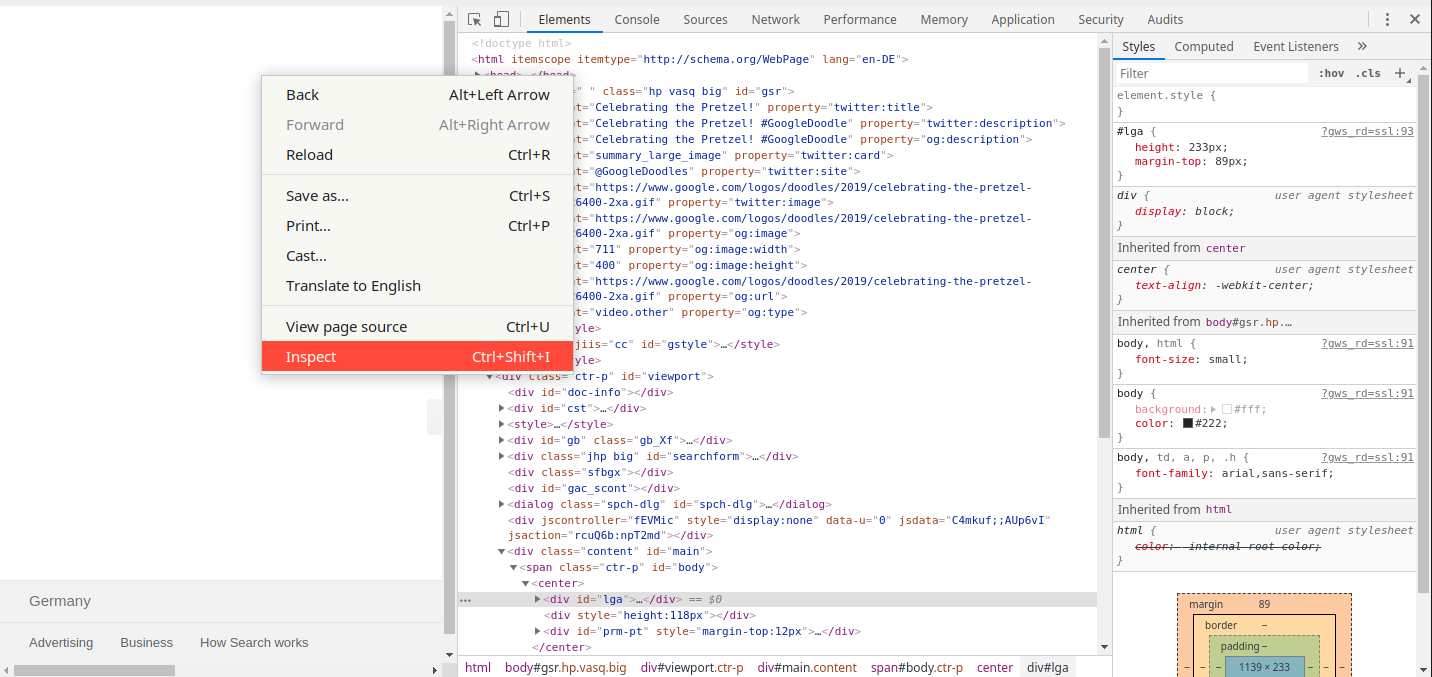
\includegraphics[width=\linewidth]{images/cdp_inspect.png}
	\caption{Zugriff auf die Chrome DevTools in Google Chrome}
	\label{scraper:image:cdpinspect}
\end{figure}

Am wichtigsten für unseren Nutzen existiert zusätzlich eine Schnittstelle, mit dem man diese DevTools algorithmisch steuern kann. Das sogenannte \ac{CDP} ermöglicht kompletten Zugriff auf die Funktionen des Google Chrome Webbrowsers sowie des Chrome DevTools. Das \ac{CDP} stellt viele hundert Funktionen zur Verfügung die auf komplexe Weise zusammenarbeiten. \cite{cdpexplorer} 

\begin{figure}[h]
	\centering
	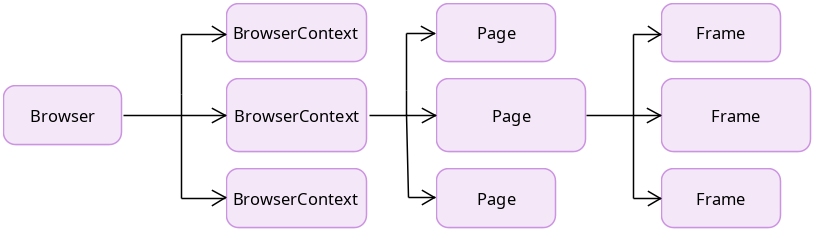
\includegraphics[]{images/cdp_overview.png}
	\caption{Struktur einer Chrome – Instanz}
	\label{scraper:image:cdptree}
\end{figure}
Abbildung \ref{scraper:image:cdptree} zeigt die Struktur einer Chrome Instanz. Das \quote{Browser} Element kann man sich als den übergeordneten Prozess vorstellen. Manchmal wird dieser auch der \quote{Allocator} genannt. Dieser Prozess besitzt dann etliche Ausführungskontexte, die größtenteils voneinander getrennt arbeiten können. Auf einem abstrakten Level kann man sie sich als verschiedene Fenster des Browsers vorstellen. Ein \quote{Fenster} hat, kann dann im Sinne von Tabs mehr als eine Seite anzeigen, welche selbst aus mindestens einem HTML Frame bestehen. \\
Wenn man mit dem \ac{CDP} entwickelt, ist es nützlich diese Struktur im Hinterkopf zu behalten. Man sollte wissen auf welcher Ebenen sich ein Funktionsaufruf auswirkt. Insbesondere können Aufrufe auch den Baum nach oben traversieren. Beispielsweise wenn ein man einen Mausklick auf einen Link im Frame simuliert, wirkt sich dieser selbstverständlich auch auf die Page aus.

%\pagebreak


Das \ac*{CDP} ist selbst in Javascript implementiert, Google empfiehlt dem normalen Entwickler es nicht direkt zu verwenden. \cite{dontuse} Für eine kleine Anwendung alle nötigen Funktionen korrekt zu verwenden sei schwer und fehleranfällig. Um auch nur einen simplen Webbrowser zu starten und zu navigieren müssen die richtigen Methoden in der richtigen Reihenfolge aufgerufen werden. Zuerst muss ein Browser erstellt oder das \ac{CDP} mit einem bestehenden Browser verbunden werden. Daraufhin müssen alle benötigten Kontexte korrekt konfiguriert werden, sodass eine Seite erstellt und navigiert werden kann. \\
Stattdessen wird geraten, vorbereitete Libraries zu verwenden, die diese komplexe Struktur abstrahieren und für die meisten Use – Cases ausreichend sind. 
\begin{table}[h]
	\centering
	\begin{tabu}{ll} \toprule
		Programmiersprache & Library \\ \midrule
		Node.js & Google Chrome Puppeteer \\
		Java & cdp4j \\
		Python & pychrome \\
		Go & chromedp, cdproto \\
		\bottomrule
	\end{tabu}
	\caption{Implementierungen des CDP}
	\label{scraper:table:cdpimpl}
\end{table}


Die obige Tabelle zeigt eine unvollständige Liste von Implementierung, die man in verschiedenen Programmiersprachen verwenden kann, um das CDP zu steuern. Wir zwei von diesen Libraries betrachten, wie wir sie verwenden können, welche Features sie bieten sowie einige Eigenartigkeiten, die uns im Projektverlauf aufgefallen sind.

\subsection*{Google Chrome Puppeteer} \label{scraper:subsec:puppeteer}
Google selbst schlägt als Abstraktion des \ac{CDP} die Verwendung ihrer eigenen Library vor. Google Chrome Puppeteer, kurz Puppeteer, ist eine Node.js API, welche die meisten Funktionen des \ac{CDP} implementiert um eine Chrome Instanz headless, oder mit einer Benutzeroberfläche zu steuern. \cite{https://pptr.dev/} Im Vergleich zur Verwendung des reinen \ac{CDP} ist Puppeteer einfach. So können wir einen neuen headless Browser starten und eine Website mit nur wenigen Zeilen laden.
\begin{minted}[frame=lines, 
framesep=2mm, 
linenos, 
baselinestretch=1.2, 
fontsize=\footnotesize]{js}
const puppeteer = require('puppeteer');

// Start a browser
const browser = await browser.launch(); 
// Create a page in the default context of this browser.
const page = await browser.newPage();  
// Navigate to a page
await page.goto('http://example.com/'); 
\end{minted}
In Hinblick auf Abbildung \ref{scraper:image:cdptree} ist auffällig, dass anscheinend kein BrowserContext erstellt werden muss. Es scheint, als ob eine Seite direkt in dem Hauptprozess / Allocator erstellt werden kann. Die ist jedoch nicht der Fall. Die Dokumentation von Puppeteer spezifiziert, dass alle Seiten in einem Standard – BrowserContext erstellt werden. Es ist zwar möglich mit der Funktion \mintinline{js}{browser.createIncognitoBrowserContext()} einen zusätzlichen Kontext anzulegen, dieser teilt aber keine Informationen mit den anderen Kontexten. Für besondere Fälle kann dies zu einem Problem werden und erfordert, dass man direkt mit dem CDP kommuniziert, um einen weiteren Kontext zu erstellen. Beispielsweise kann es sein, dass man in zwei Kontexten auf der gleichen Seite arbeiten möchte. Dies hat den Vorteil, dass man beide Kontexte parallel bearbeiten kann, während Informationen wie Cookies mit Login Daten zwischen den Kontexten geteilt werden. \footnote{Dies ist uns in der Implementierung passiert, da wir PDFs und Screenshots parallel rendern wollten.} \\
Nun können wir den HTML Renderer von Google Chrome nutzen um Screenshots und PDF Dateien herzustellen:  
\begin{minted}[frame=lines, 
framesep=2mm, 
linenos, 
baselinestretch=1.2, 
fontsize=\footnotesize]{js}
await page.screenshot({path : 'example.png'});
await page.pdf({path : 'example.pdf'});
\end{minted}